\documentclass[a4paper,10pt]{article}

\usepackage[T1]{fontenc}
\usepackage[utf8]{inputenc}
\usepackage{graphicx}
\usepackage{xcolor}
\usepackage{fourier}
\usepackage{caption}
\usepackage{subcaption}
\usepackage{cprotect}

\usepackage{tgtermes}

\usepackage[
pdftitle={Statistical Machine Learning}, 
pdfauthor={Inez Wijnands \& Guido Zuidhof, Radboud University Nijmegen},
colorlinks=true,linkcolor=blue,urlcolor=blue,citecolor=blue,bookmarks=true,
bookmarksopenlevel=2]{hyperref}
\usepackage{amsmath,amssymb,amsthm,textcomp}
\usepackage{enumerate}
\usepackage{multicol}
\usepackage{tikz}

\usepackage{geometry}
\geometry{total={210mm,297mm},
left=25mm,right=25mm,%
bindingoffset=0mm, top=20mm,bottom=20mm}

\numberwithin{equation}{section} % Number equations within sections (i.e. 1.1 instead of 1)
\numberwithin{figure}{section} % Number figures within sections (i.e. 1.1 i/o 1)
\numberwithin{table}{section} % Number tables within sections (i.e. 1.1 i/of 1)

\linespread{1.35}

\newcommand{\linia}{\rule{\linewidth}{0.5pt}}

% custom theorems if needed
\newtheoremstyle{mytheor}
    {1ex}{1ex}{\normalfont}{0pt}{\scshape}{.}{1ex}
    {{\thmname{#1 }}{\thmnumber{#2}}{\thmnote{ (#3)}}}

\theoremstyle{mytheor}
\newtheorem{defi}{Definition}

% my own titles
\makeatletter
\renewcommand{\maketitle}{
\begin{center}
\vspace{2ex}
{\huge \textsc{\@title}}
\vspace{1ex}
\\
\linia\\
\@author  \@date
\vspace{4ex}
\end{center}
}
\makeatother
%%%

% custom footers and headers
\usepackage{fancyhdr,lastpage}
\pagestyle{fancy}
\lhead{}
\chead{}
\rhead{}
\lfoot{Assignment \textnumero{} 4}
\cfoot{}
\rfoot{Page \thepage\ /\ \pageref*{LastPage}}
\renewcommand{\headrulewidth}{0pt}
\renewcommand{\footrulewidth}{0pt}
%

% code listing settings
\usepackage{listings}
\lstset{
    language=Python,
    basicstyle=\ttfamily\small,
    aboveskip={0.9\baselineskip},
    belowskip={0.9\baselineskip},
    columns=fixed,
    extendedchars=true,
    breaklines=true,
    tabsize=4,
    prebreak=\raisebox{0ex}[0ex][0ex]{\ensuremath{\hookleftarrow}},
    frame=lines,
    showtabs=false,
    showspaces=false,
    showstringspaces=false,
    keywordstyle=\color[rgb]{0.1,0.126,0.941},
    commentstyle=\color[rgb]{0.133,0.545,0.133},
    stringstyle=\color[rgb]{0,0.5,0},
    numbers=left,
    numberstyle=\scriptsize\ttfamily,
    stepnumber=1,
    numbersep=10pt,
    captionpos=t,
    escapeinside={\%*}{*)}
}

%%%----------%%%----------%%%----------%%%----------%%%

\begin{document}

\title{Statistical Machine Learning \\ Assignment 4}

\author{Inez Wijnands (s4149696) \& Guido Zuidhof (s4160703)\\ Radboud University Nijmegen\\}

\date{18/01/2015}

\maketitle

\noindent \textit{The entire code listing is included in the zip-file. The listings shown here are merely code snippets}.\vspace{-0.5cm}
\section{Neural networks}
\begin{enumerate}
	\item Since all the weights have the same update function, if all the weights are $0$,  after the updates they will still remain the same as the other weights. This way you don't break the symmetry when backpropagating.
	\item First, we take the weighted sum of the input $x$:
		\begin{align*}
		a_j &= \sum_i w_{ji}x_i + b_j^{(1)} x_0\\
		a_1 &= w_{1}^{(1)} \cdot x_1 + b_{1}^{(1)} \cdot x_0 = 0.5 + 1 = 1.5\\
		a_2 &= w_{2}^{(1)} \cdot x_1 + b_{2}^{(1)} \cdot x_0 = 0.05 + 0 = 0.05 \\
		a_3 &= w_{3}^{(1)} \cdot x_1 + b_{3}^{(1)} \cdot x_0 = -0.5 + 1 = 0.5
		\end{align*}
		\noindent Where the input $x_i$ given in the assignment $\in \{x_1,t_1\} = \{0.5, 0.25\}$, and $w_{ji}$ is also given $\in w^{(1)} = [1,0.1,-1]$.\\
		Now we calculate the activation $z_j$ of unit $j$:
		\begin{align*}
		z_j &= h(a_j) = \tanh(a_j) = \frac{e^{a_j} - e^{-a_j}}{e^{a_j} + e^{-a_j}}\\
		z_1 &= \tanh(1.5) = 0.90515\\
		z_2 &= \tanh(0.05) = 0.04996\\
		z_3 &= \tanh(0.5) = 0.46212
		\end{align*}
		Then, we calculate the output using the linear activation function given in the assignment:
		\begin{align*}
		y &= \sum_j w_j^{(2)}z_j + b_1^{(2)}\\
		&= w_1^{(2)}z_1 + w_2^{(2)}z_2 + w_3^{(2)}z_3 + b_1^{(2)}\\
		&= -1 \cdot 0.90515 + 0.1 \cdot 0.04996 + -1 \cdot 0.46212 + 2\\
		&= -0.90515 + 0.004996 - 0.46212 + 2 \\
		&= 0.63773
		\end{align*}
		Second, we backpropagate the error $\delta = (y - t)$ to establish the derivatives $\frac{\partial E}{\partial w_{ji}}$, using a standard sum-of-squares function (with $K = 1$ since there is only one output value):
		\begin{align*}
		\delta_k &= y_k - t_k\\
		E_n &= \frac{1}{2} \sum_1^K \delta_k^2\\
		&= \frac{1}{2} \cdot (0.63773 - 0.25)^2 = \frac{1}{2} \cdot 0.37227^2 = \frac{1}{2} \cdot 0.15033 = 0.07517
		\end{align*}
		Then we backpropagate these $\delta$'s for the hidden units:
		\begin{align*}
		\delta_j \hspace{0.2cm} &= h'(a_j) \sum_1^K w_{kj} \delta_k\\
			 &= (1 - h(a_j)^2) \sum_1^K w_{kj} \delta_k\\
			 &= (1 - z_j^2) \sum_1^K w_{kj} \delta_k\\
		\delta_1\hspace{0.2cm}  &= (1 - z_1^2) \cdot w_{1}^{(2)} \cdot 0.37227\\
			 &= (1 - 0.90515^2) \cdot -1 \cdot 0.37227\\
			 &= (1 - 0.81930) \cdot -0.37227\\
			 &= 0.18070 \cdot -0.37227 = -0.06727\\
		\delta_2 \hspace{0.2cm} &= (1 - z_2^2) \cdot w_{2}^{(2)} \cdot 0.37227\\
			 &= (1 - 0.04996^2) \cdot 0.1 \cdot 0.37227\\
			 &= (1 - 0.00250) \cdot 0.03723\\
			 &= 0.99750 \cdot 0.03723 = 0.03714\\
		\delta_3 \hspace{0.2cm} &= (1 - z_3^2) \cdot w_{3}^{(2)} \cdot 0.37227\\
			 &= (1 - 0.46212^2) \cdot -1 \cdot 0.37227\\
			 &= (1 - 0.21355) \cdot -0.37227\\
			 &= 0.78645 \cdot -0.37227 = -0.29277
		\end{align*}
		Third, the derivatives with respect to the first-layer and second-layer weights are given by:
		\begin{align*}
		\frac{\partial E_n}{\partial w_{ji}^{(1)}} = \delta_j x_i = \Delta w_{j}^{(1)} & & & & \frac{\partial E_n}{\partial w_{kj}^{(2)}} = \delta_k z_j = \Delta w_{j}^{(2)} \hspace{2cm}\\
		 \Delta w_{1}^{(1)} = -0.06727 \cdot 0.5 = -0.03364 & & & &  \Delta w_{1}^{(2)}  = 0.37277 \cdot 0.90515 = 0.33741\\
		 \Delta w_{2}^{(1)} = \hspace{0.2cm} 0.03714 \cdot 0.5 = \hspace{0.2cm} 0.01857	& & & &   \Delta w_{2}^{(2)}  = 0.37227 \cdot 0.04996 = 0.01862 \\
		  \Delta w_{3}^{(1)} = -0.29277 \cdot 0.5 = -0.14639 & & & &   \Delta w_{3}^{(2)} = 0.37277 \cdot 0.46212 = 0.17226 
		\end{align*}
		And to update the weights, we use learning rate $\eta = 0.5$:
		\begin{align*}
		w_1^{(1)} &:= w_1^{(1)} - \eta \Delta w_1^{(1)} = 1 - 0.5 \cdot -0.03364 = 1.01682\\
		w_2^{(1)} &:= w_2^{(1)} - \eta \Delta w_2^{(1)} = 0.1 - 0.5 \cdot 0.01857 = 0.09072\\	
		w_3^{(1)} &:= w_3^{(1)} - \eta \Delta w_3^{(1)} = -1 - 0.5 \cdot -0.14639 = -0.92681\\	
		w_1^{(2)} &:= w_1^{(2)} - \eta \Delta w_1^{(2)} = -1 - 0.5 \cdot 0.33741 = -1.16871\\
		w_2^{(2)} &:= w_2^{(2)} - \eta \Delta w_2^{(2)} = 0.1 - 0.5 \cdot 0.01862 = 0.09159 \\
		w_3^{(2)} &:= w_3^{(2)} - \eta \Delta w_3^{(2)} = -1 - 0.5 \cdot 0.17226 = -1.08613
		\end{align*}
		Last, to check whether or not the updated network has improved the output (i.e. has a smaller error), we recalculate the first step given the same input.\\
		We recalculate the weighted sum of the input with the new weights and use the activation function to obtain $z_j$:
		\begin{align*}
		z_1 &= \tanh w_{1}^{(1)} \cdot x_1 + b_{1}^{(1)} \cdot x_0 = \tanh(1.01682 \cdot 0.5 + 1 \cdot 1) = \tanh(1.50841) = 0.90666\\
		z_2 &= \tanh w_{2}^{(1)} \cdot x_1 + b_{2}^{(1)} \cdot x_0 = \tanh(0.09072 \cdot 0.5 + 0 \cdot 1) = \tanh(0.04536) = 0.04533\\
		z_3 &= \tanh w_{3}^{(1)} \cdot x_1 + b_{3}^{(1)} \cdot x_0 = \tanh(-0.92681 \cdot 0.5 + 1 \cdot 1) = \tanh(0.53660) = 0.49041
		\end{align*}
		We recalculate the output with the new activations:
		\begin{align*}
		y &= \sum_j w_j^{(2)}z_j + b_1^{(2)}\\
		&= w_1^{(2)}z_1 + w_2^{(2)}z_2 + w_3^{(2)}z_3 + b_1^{(2)}\\
		&= -1.16871 \cdot 0.90666 + 0.09159 \cdot 0.04533 + -1.08613 \cdot 0.49041 + 2\\
		&= 0.41188
		\end{align*}
		If we repeat the second step, we obtain the new error:
		\begin{align*}
		\delta_k &= y_k - t_k\\
		E_n &= \frac{1}{2} \sum_1^K \delta_k^2\\
		&= \frac{1}{2} \cdot (0.41188 - 0.25)^2 = \frac{1}{2} \cdot 0.16188^2 = \frac{1}{2} \cdot 0.02621 = 0.01310
		\end{align*}
		The sum-of-squares error of the output is smaller than the previous error. Thus, it has improved.		
	\item If you only use linear activation functions for the hidden layer nodes, the network cannot model nonlinear combinations of the inputs. If the classification problem is not linearly separable, no matter how many hidden nodes you have, you can still only obtain linear separations and thus not solve this problem very well.
	\item Due to the fairly high noise in the data we can not be very certain that it will converge. The sequential procedure is quite susceptible to noise, as for instance sequential points with high noise with the same sign may make for weights moving far away from an optimum. The batch procedure is less susceptible to this problem, as the noise gets averaged out for all 50 points.\\
\\
The weights of either approach do not have to end up with the same final weight distribution.
\end{enumerate}

%\vfill 

\section{Neural network regression}
\begin{enumerate}
	\item \begin{figure}[h]
   			\centering
   			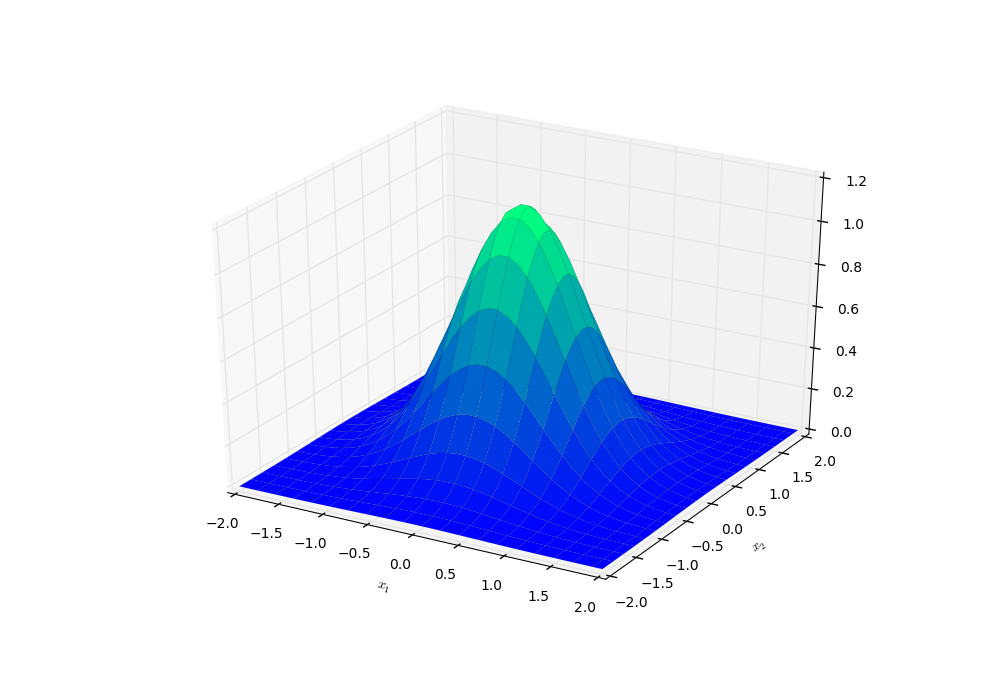
\includegraphics[width=0.88\textwidth]{std_iso_gaussian.png}\vspace{-1cm}
   			\caption{\vspace{-0.1cm} Isotropic 2D Gaussian $y = 3 \cdot \mathcal{N}(\boldsymbol{x} \big\vert \boldsymbol{0}, \frac{2}{5} \boldsymbol{I}_2)$.}\vspace{-0.2cm}
  		\end{figure}
	\item We have used the activation functions of the previous exercise. We also introduced a bias node in the input layer and in the hidden layer, similar to the previous exercise. The weights for these biases are initialized randomly, the same as the other weights in our network. 
		\begin{figure}[h!]
			\centering
			\begin{subfigure}[b]{0.45\textwidth}
				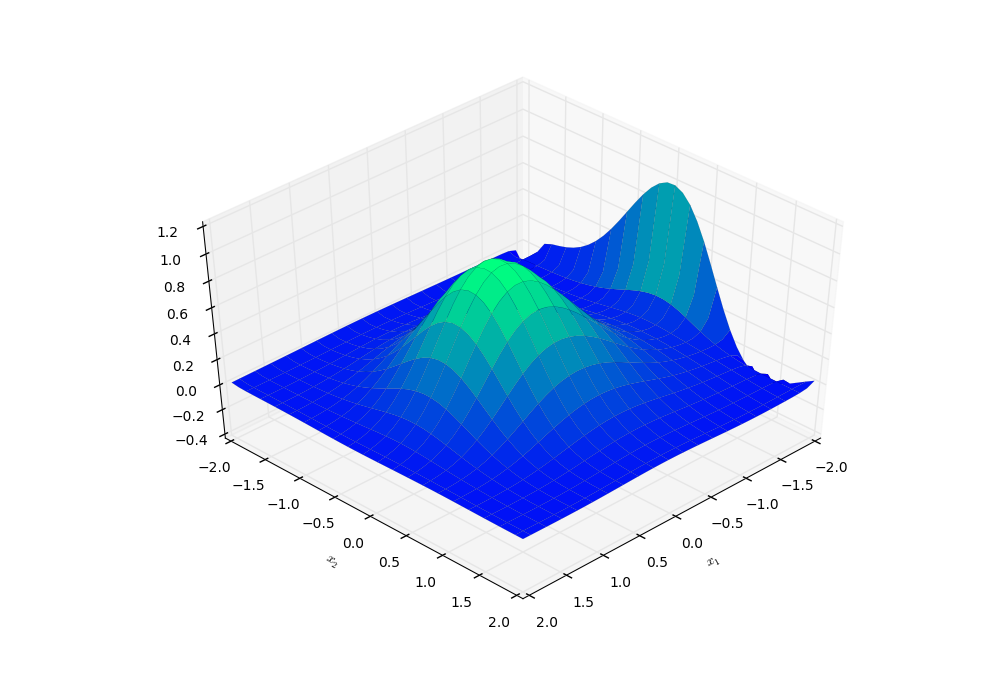
\includegraphics[width=\textwidth]{ex2_2.png}\vspace{-0.5cm}
				\caption{Initial output.}
			\end{subfigure}
			\begin{subfigure}[b]{0.45\textwidth}
				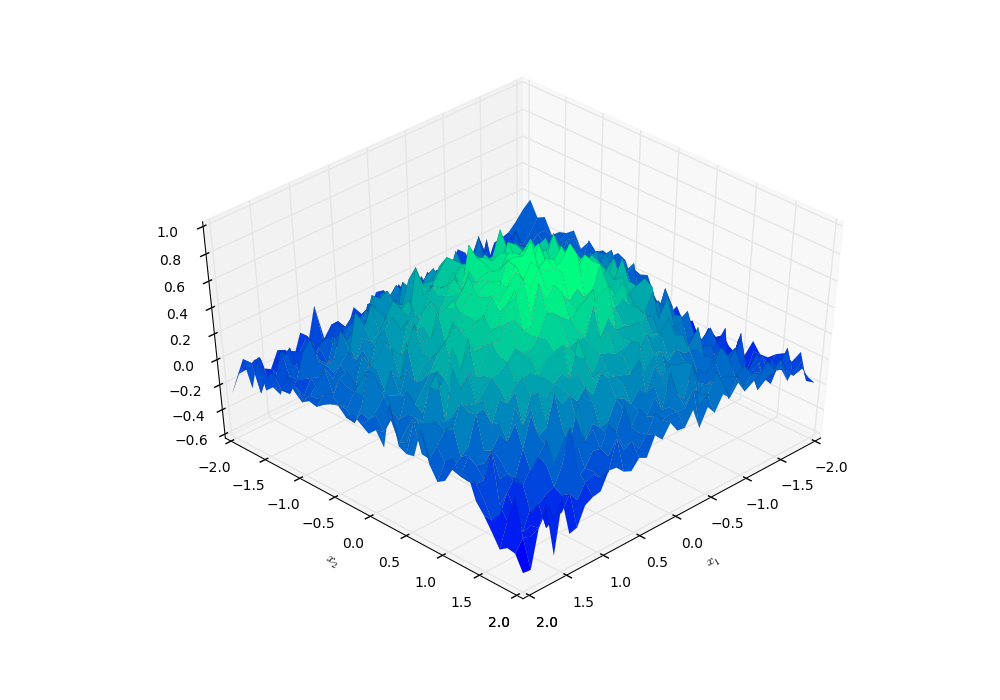
\includegraphics[width=\textwidth]{ex2_2_1.png}\vspace{-0.5cm}
				\caption{Output of the second cycle.}
			\end{subfigure}
   			\caption{\vspace{-0.1cm} 2D graphs of initial output of network.}\vspace{-0.2cm}
  		\end{figure}
	\item \begin{figure}[h!]
			\centering
			\begin{subfigure}[b]{0.45\textwidth}
				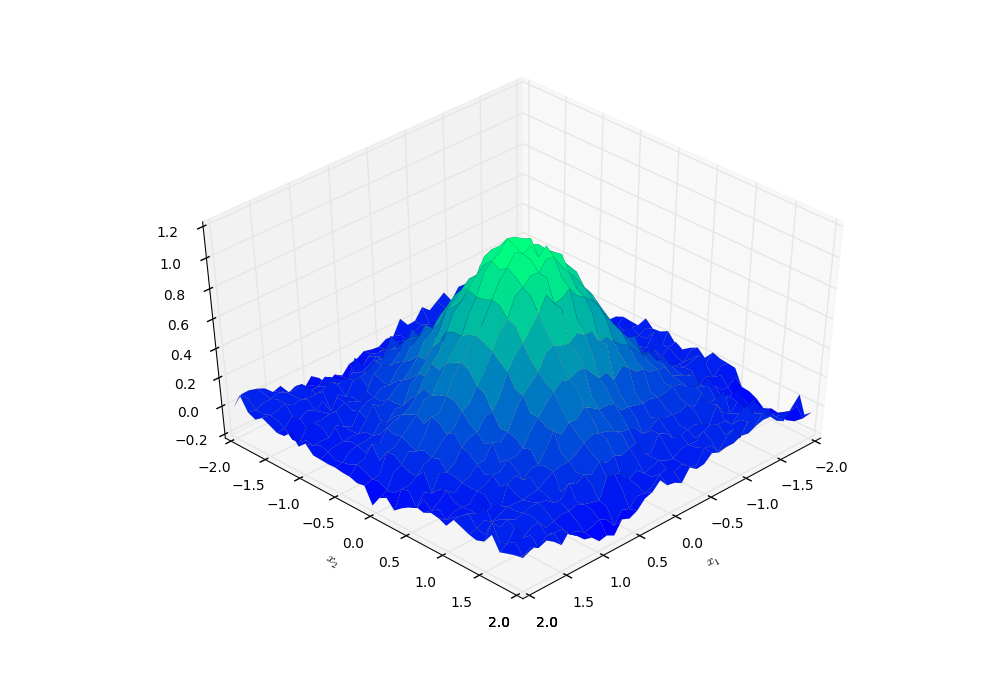
\includegraphics[width=\textwidth]{ex2_3_50.png}\vspace{-0.5cm}
				\caption{Output after 50 cycles.}
			\end{subfigure}
			\begin{subfigure}[b]{0.45\textwidth}
				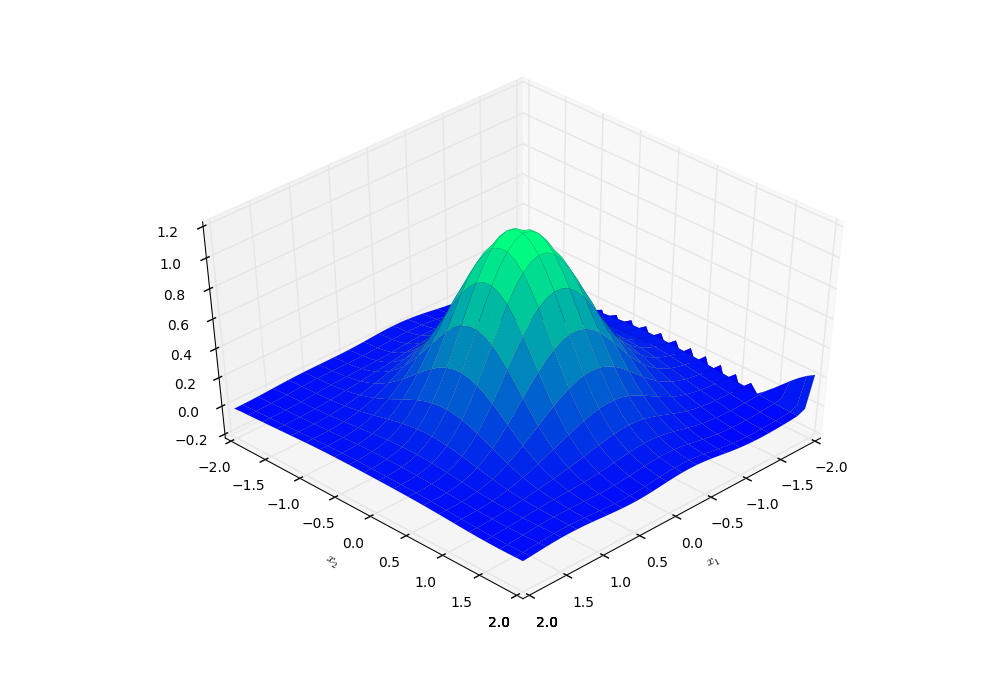
\includegraphics[width=\textwidth]{ex2_3_100.png}\vspace{-0.5cm}
				\caption{Output after 100 cycles.}
			\end{subfigure}
			\begin{subfigure}[b]{0.45\textwidth}
				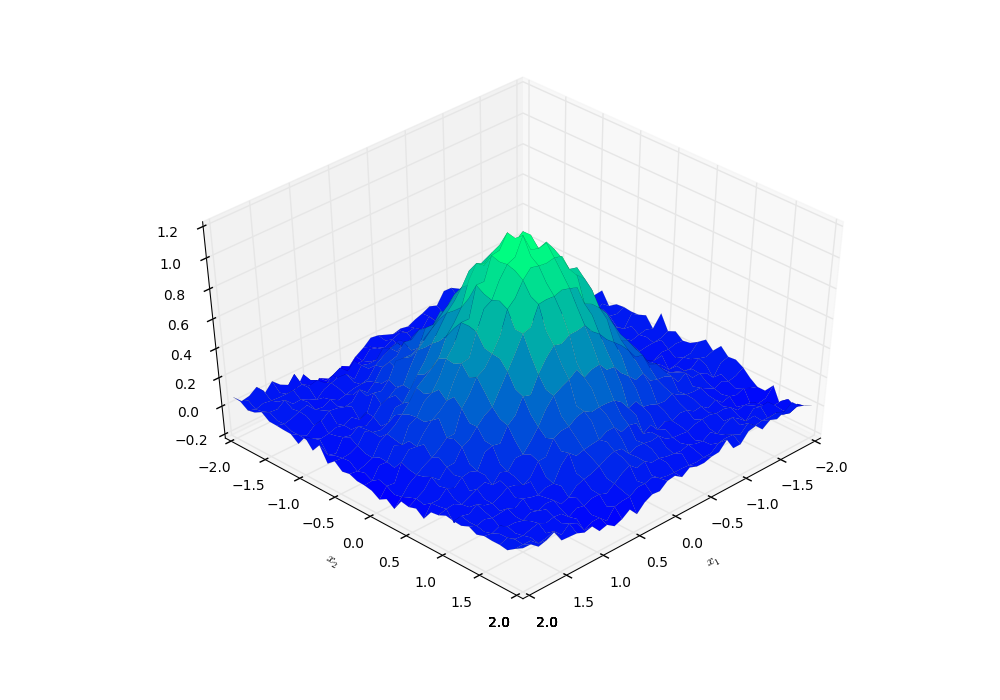
\includegraphics[width=\textwidth]{ex2_3_200.png}\vspace{-0.5cm}
				\caption{Output after 200 cycles.}
			\end{subfigure}
			\begin{subfigure}[b]{0.45\textwidth}
				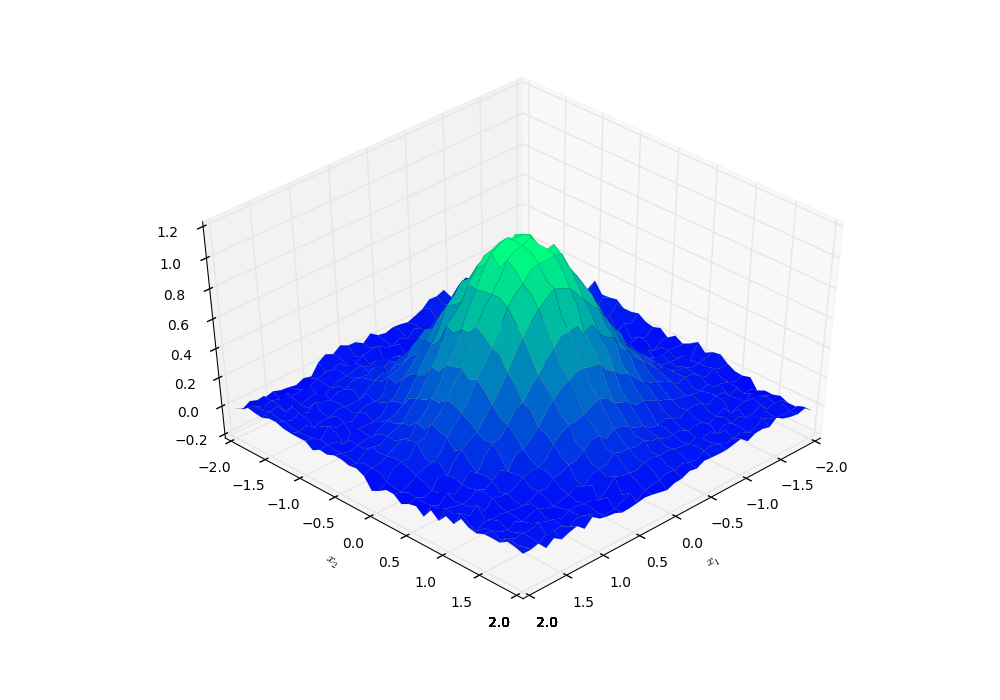
\includegraphics[width=\textwidth]{ex2_3_500.png}\vspace{-0.5cm}
				\caption{Output after 500 cycles.}
			\end{subfigure}
   			\caption{\vspace{-0.1cm} 2D graphs of the output of network.}\vspace{-0.2cm}
  		\end{figure}
		In Figure 2.2 and Figure 2.3 is shown that the initial outputs still contain multiple peaks. After 100 cycles the output is nearly converged, only really small changes are visible. The plot already resembles the Gaussian density shown in Figure 2.1. Although the expected wobbles are not present.
	\item \begin{figure}[h!]
			\centering
			\begin{subfigure}[b]{0.45\textwidth}
				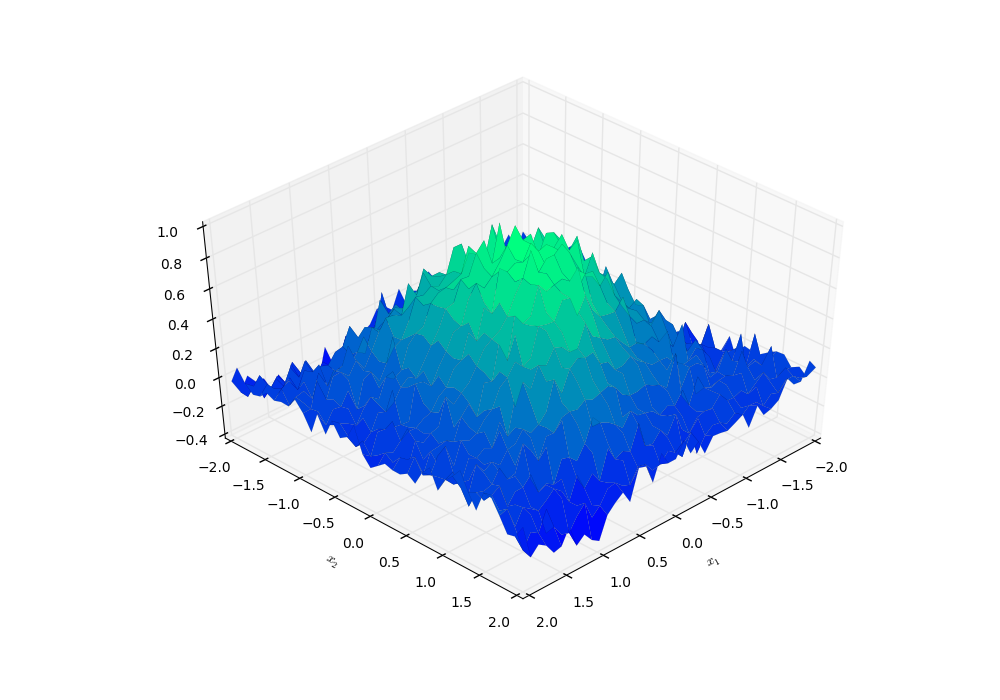
\includegraphics[width=\textwidth]{ex2_4_10.png}\vspace{-0.5cm}
				\caption{Output after 10 cycles.}
			\end{subfigure}
			\begin{subfigure}[b]{0.45\textwidth}
				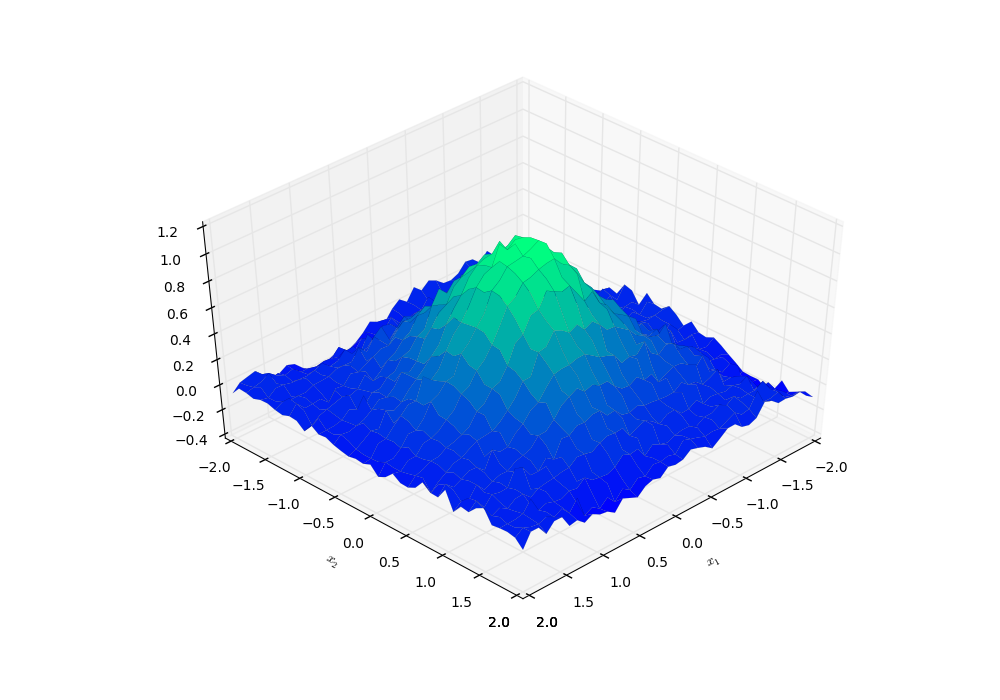
\includegraphics[width=\textwidth]{ex2_4_30.png}\vspace{-0.5cm}
				\caption{Output after 30 cycles.}
			\end{subfigure}
			\begin{subfigure}[b]{0.45\textwidth}
				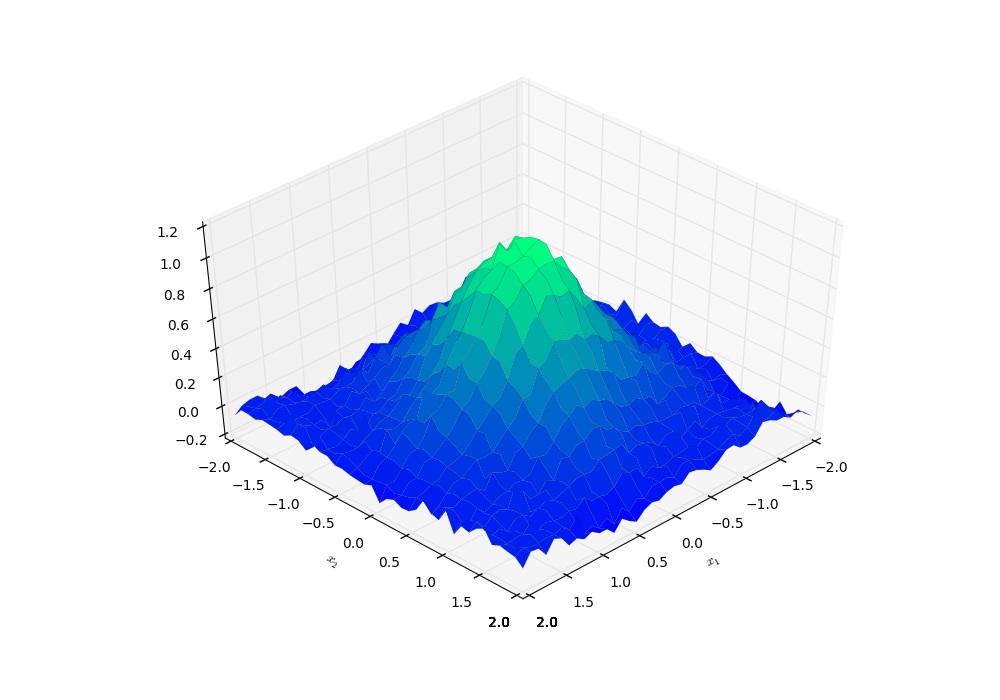
\includegraphics[width=\textwidth]{ex2_4_50.png}\vspace{-0.5cm}
				\caption{Output after 50 cycles.}
			\end{subfigure}
			\begin{subfigure}[b]{0.45\textwidth}
				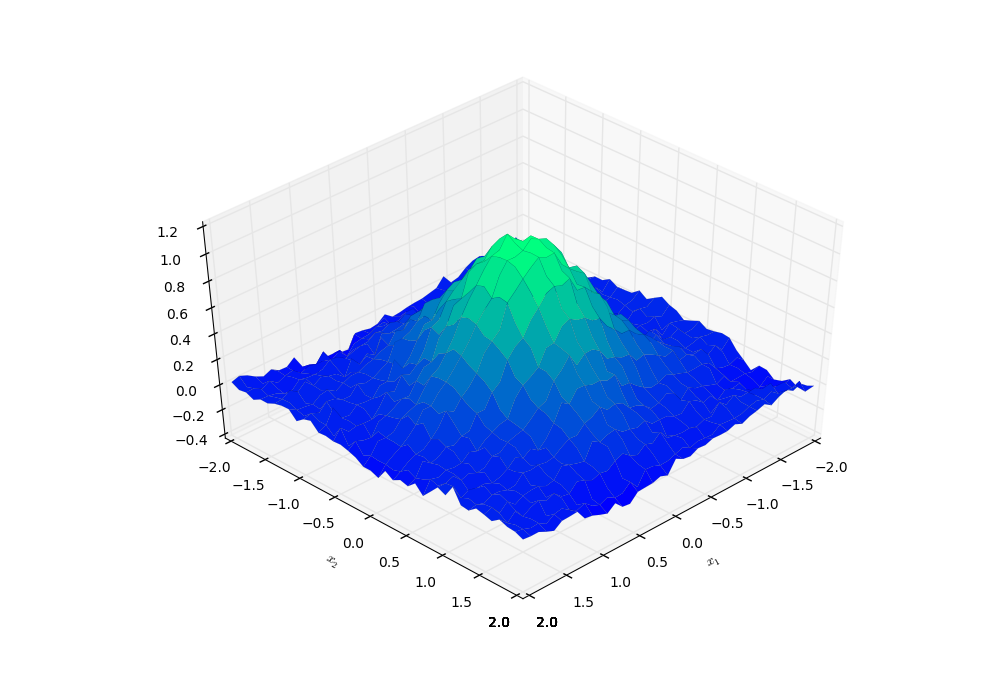
\includegraphics[width=\textwidth]{ex2_4_80.png}\vspace{-0.5cm}
				\caption{Output after 80 cycles.}
			\end{subfigure}
			\begin{subfigure}[b]{0.45\textwidth}
				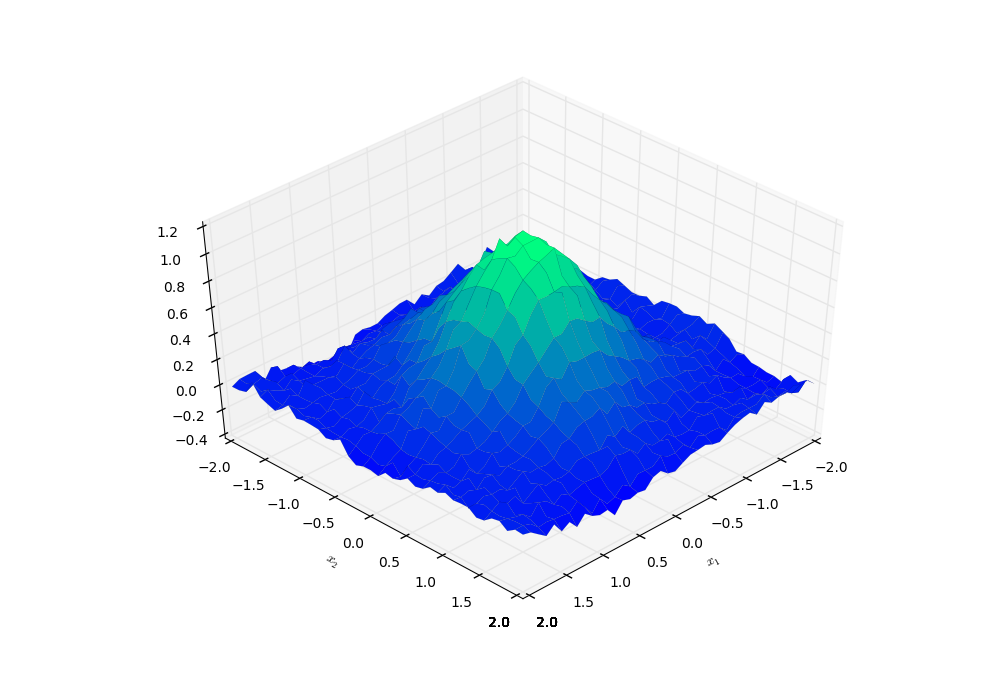
\includegraphics[width=\textwidth]{ex2_4_100.png}\vspace{-0.5cm}
				\caption{Output after 100 cycles.}
			\end{subfigure}
			\begin{subfigure}[b]{0.45\textwidth}
				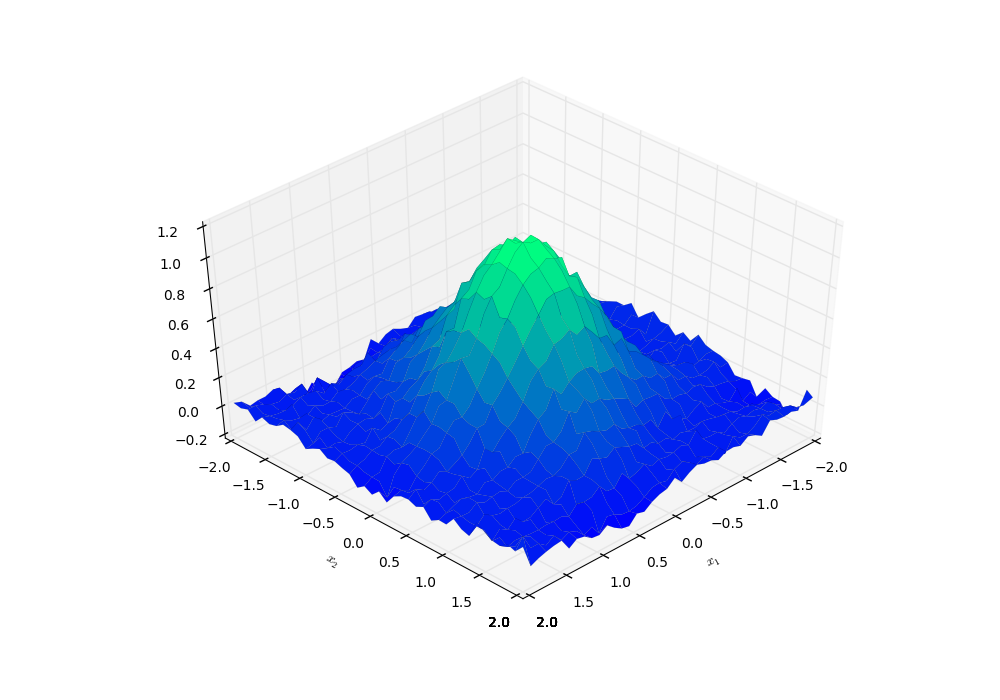
\includegraphics[width=\textwidth]{ex2_4_500.png}\vspace{-0.5cm}
				\caption{Output after 500 cycles.}
			\end{subfigure}
   			\caption{\vspace{-0.1cm} 2D graphs of the output of network where the data set is in a randomized order}\vspace{-0.2cm}
  		\end{figure}
		\noindent In Figure 2.4 is shown what the output looks like when the dataset is permuted in a random order. Convergence is established after around 50-80 cycles, so a bit faster than in 2.3. However, we do see the wobbles in these plots, while we expected to see them as well in 2.3.\\\\
		Second, we trained the network using 16 hidden nodes instead of 8, but we did not see much difference. However,  the network takes more time to train. When we tried 4 hidden nodes, the network performed quite badly, as can be seen in Figure 2.5. The ouput does not change after more cycles, thus convergence is fast.
		\begin{figure}[h!]
   			\centering
   			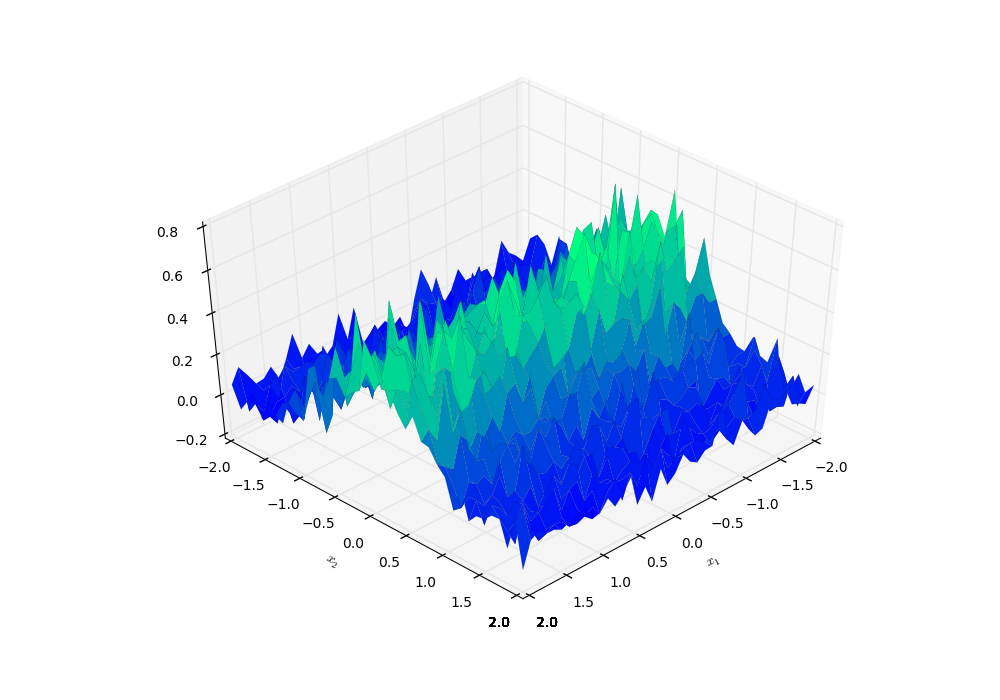
\includegraphics[width=0.44\textwidth]{ex2_4lh_500.png}\vspace{-0.6cm}
   			\caption{\vspace{-0.1cm} 2D graphs of the output of network after 500 cycles with a randomized data order, 4 hidden nodes}\vspace{-0.2cm}
  		\end{figure}
		
		When we change the learning rate to 0.01 instead of 0.1, we get a smoother plot. Convergence is slower, around 250 cycles, as is shown in Figure 2.6.\\
		\begin{figure}[h!]
			\centering
			\begin{subfigure}[b]{0.45\textwidth}
				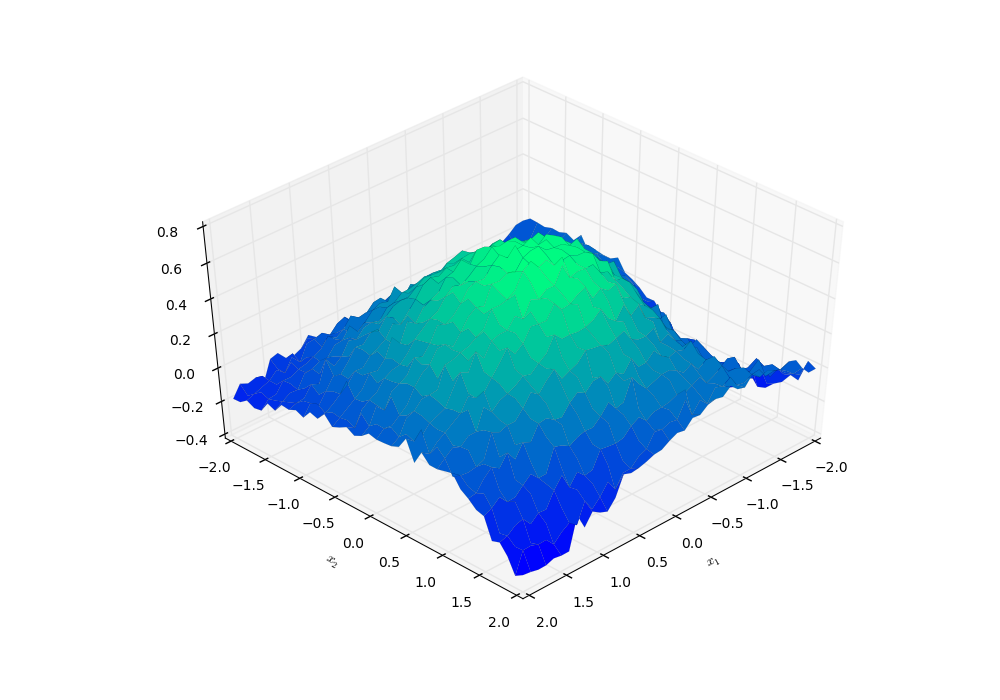
\includegraphics[width=\textwidth]{ex2_4llr_10.png}\vspace{-0.5cm}
				\caption{Output after 10 cycles.}
			\end{subfigure}
			\begin{subfigure}[b]{0.45\textwidth}
				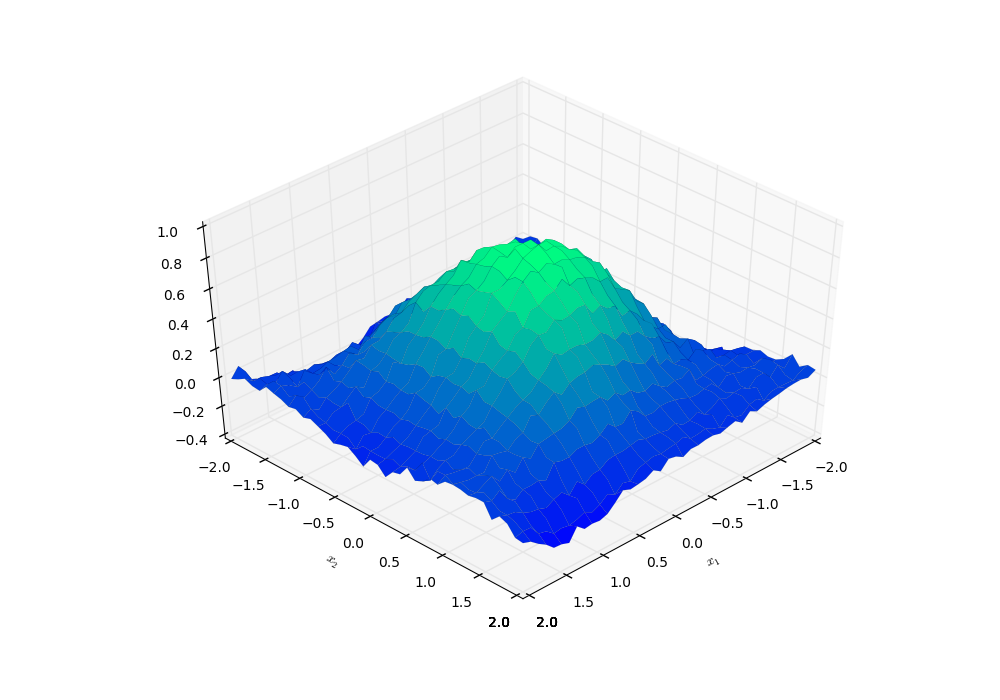
\includegraphics[width=\textwidth]{ex2_4llr_50.png}\vspace{-0.5cm}
				\caption{Output after 50 cycles.}
			\end{subfigure}
			\begin{subfigure}[b]{0.45\textwidth}
				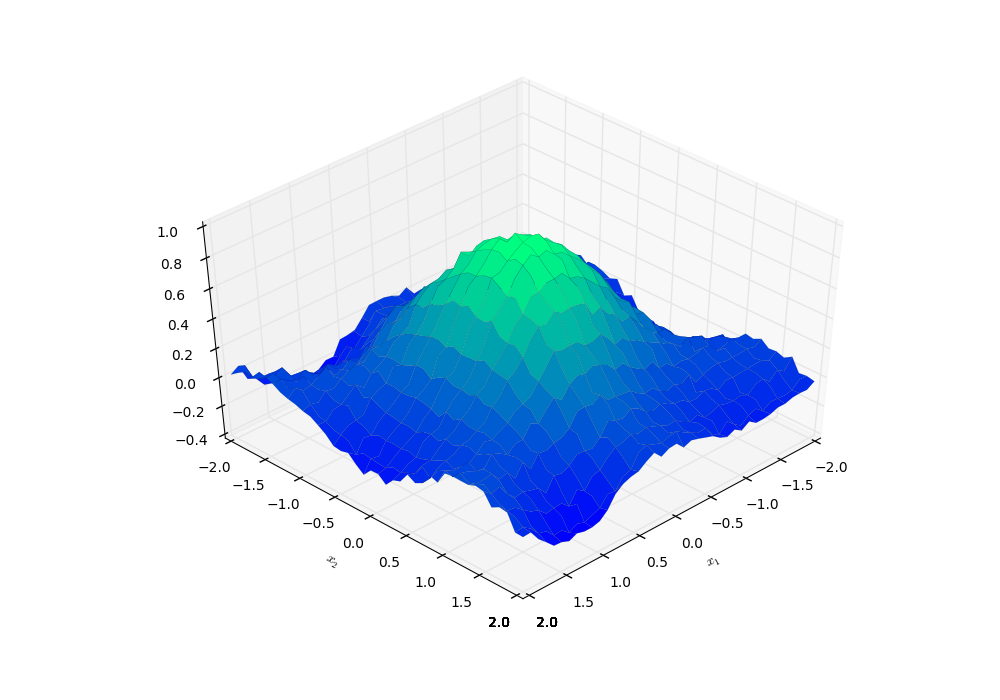
\includegraphics[width=\textwidth]{ex2_4llr_100.png}\vspace{-0.5cm}
				\caption{Output after 100 cycles.}
			\end{subfigure}
			\begin{subfigure}[b]{0.45\textwidth}
				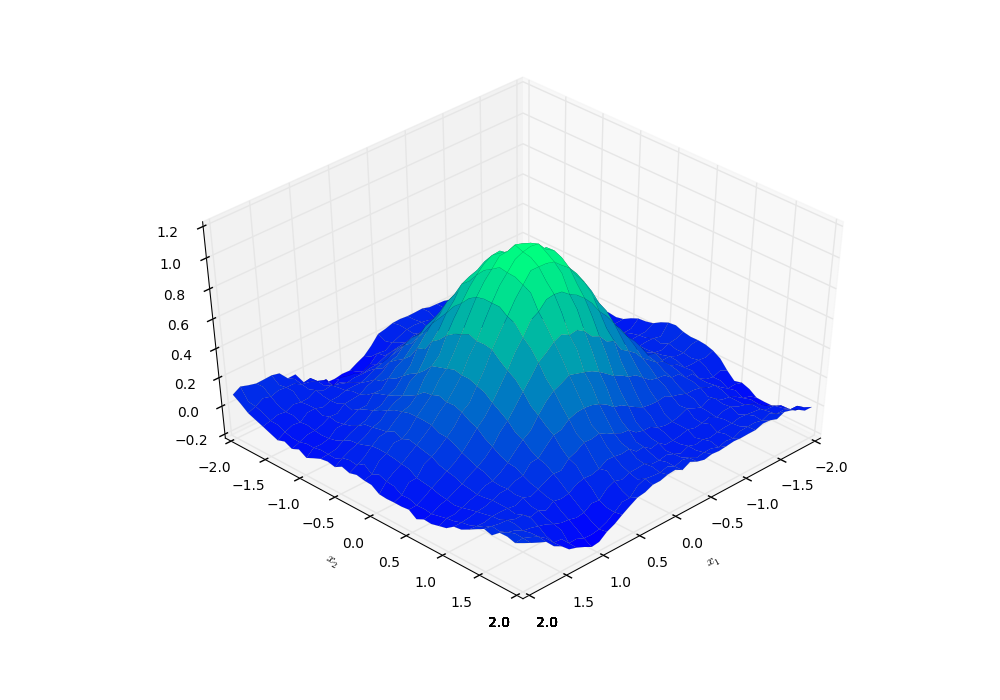
\includegraphics[width=\textwidth]{ex2_4llr_200.png}\vspace{-0.5cm}
				\caption{Output after 200 cycles.}
			\end{subfigure}
			\begin{subfigure}[b]{0.45\textwidth}
				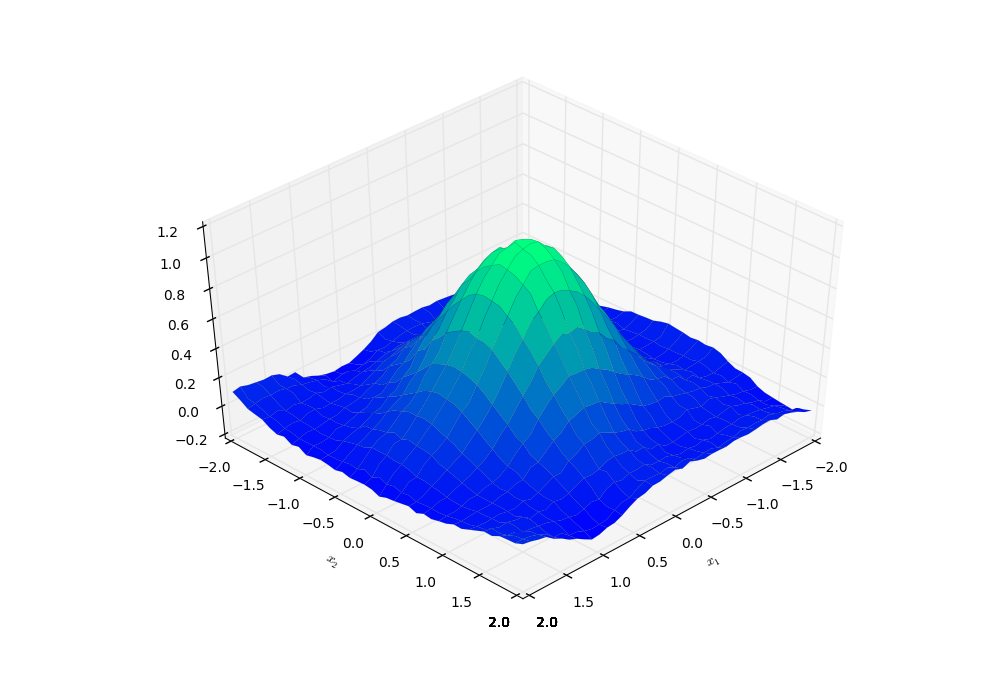
\includegraphics[width=\textwidth]{ex2_4llr_300.png}\vspace{-0.5cm}
				\caption{Output after 300 cycles.}
			\end{subfigure}
			\begin{subfigure}[b]{0.45\textwidth}
				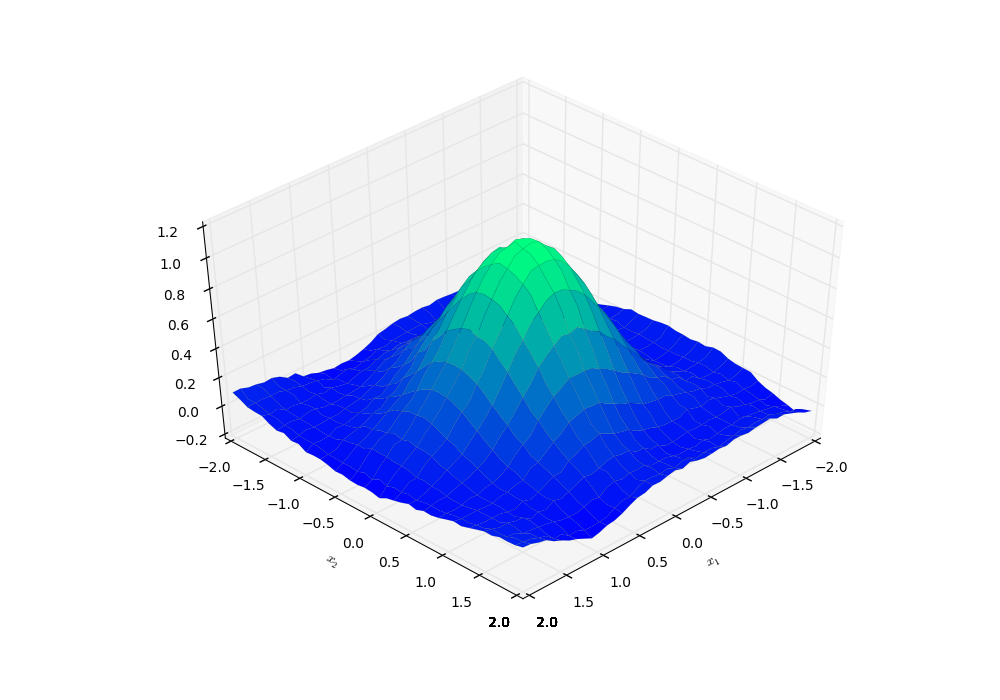
\includegraphics[width=\textwidth]{ex2_4llr_500.png}\vspace{-0.5cm}
				\caption{Output after 500 cycles.}
			\end{subfigure}
   			\caption{\vspace{-0.1cm} 2D graphs of the output of network where the data set is in a randomized order, with $\eta = 0.01$}\vspace{-0.2cm}
  		\end{figure}
		
	\item \begin{figure}[h!]
   			\centering
   			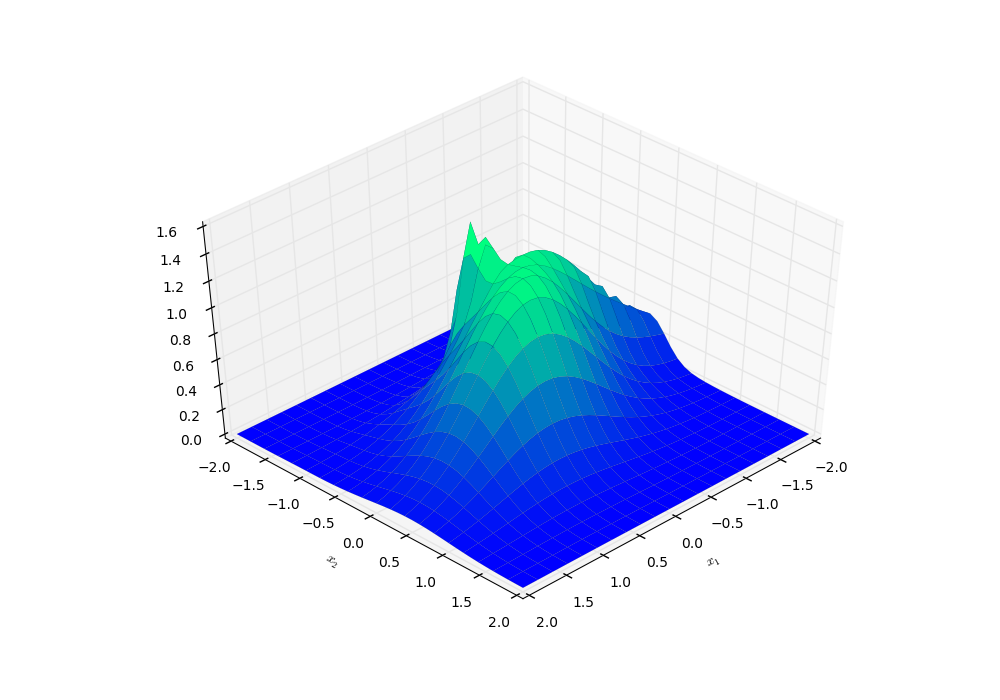
\includegraphics[width=0.44\textwidth]{ex2_5.png}\vspace{-0.6cm}
   			\caption{\vspace{-0.1cm} 2D graph of the target probability density function of the real data}\vspace{-0.2cm}
  		\end{figure}
	\item We used 60 hidden nodes, and a learning rate of 0.001, for 2000 cycles. The output is almost converged after around 200-300 cycles, only changing a bit towards 2000 cycles.
		\begin{figure}[h!]
			\centering
			\begin{subfigure}[b]{0.45\textwidth}
				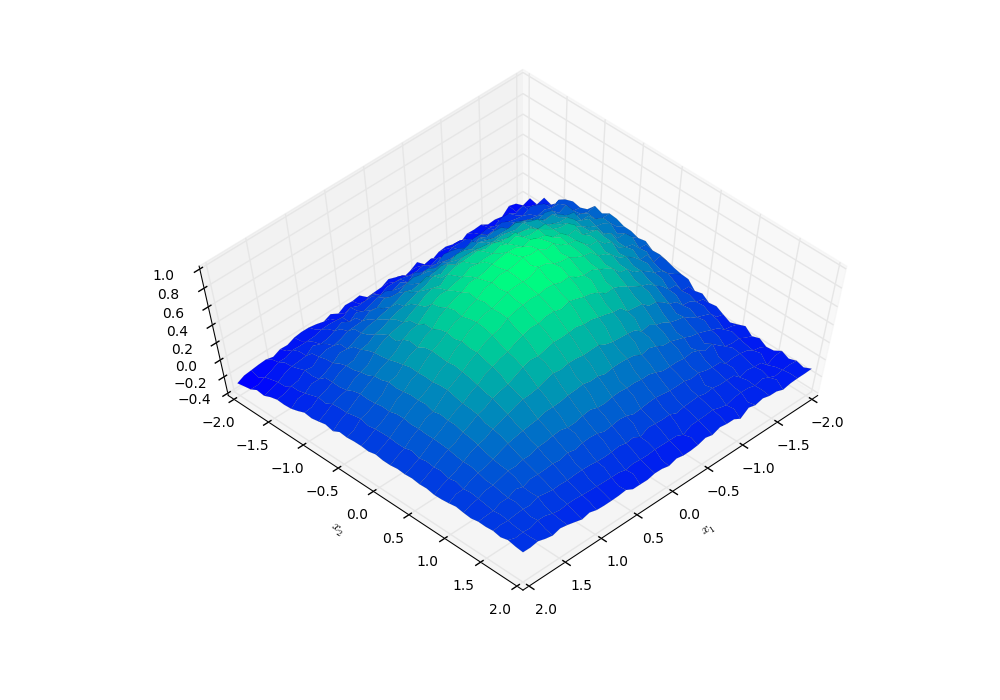
\includegraphics[width=\textwidth]{plot/ex2_6_50.png}\vspace{-0.5cm}
				\caption{Output after 50 cycles.}
			\end{subfigure}
			\begin{subfigure}[b]{0.45\textwidth}
				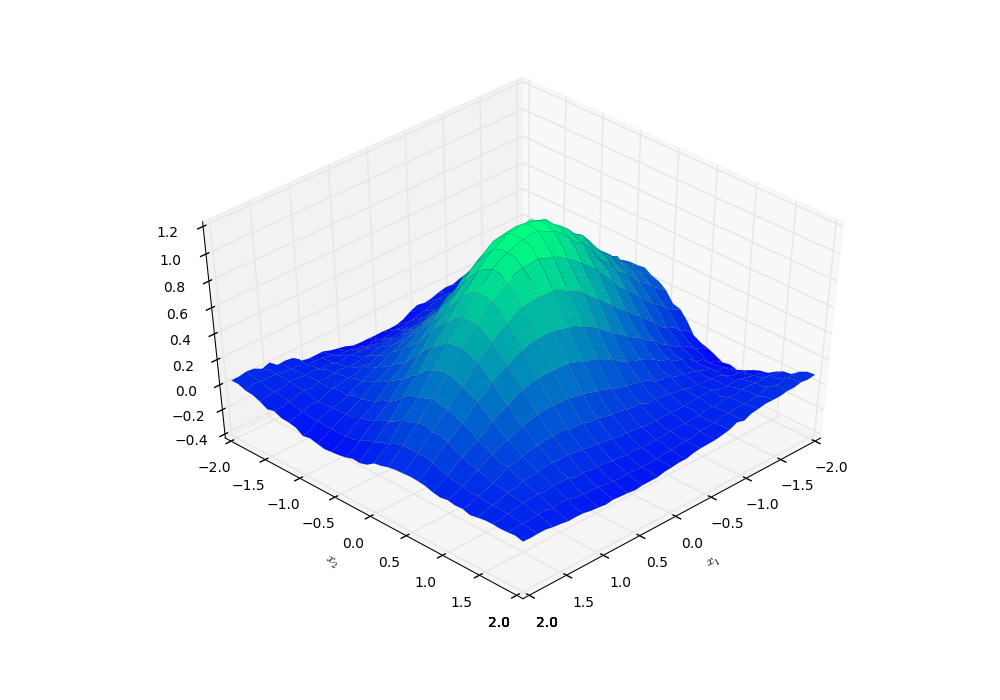
\includegraphics[width=\textwidth]{plot/ex2_6_200.png}\vspace{-0.5cm}
				\caption{Output after 200 cycles.}
			\end{subfigure}
			\begin{subfigure}[b]{0.45\textwidth}
				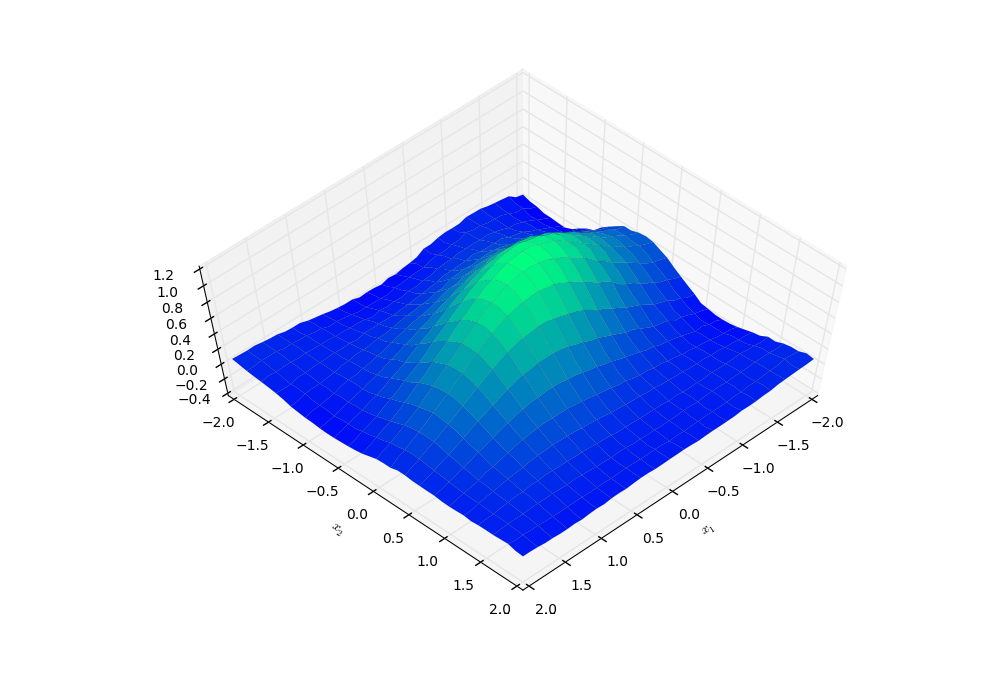
\includegraphics[width=\textwidth]{plot/ex2_6_300.png}\vspace{-0.5cm}
				\caption{Output after 300 cycles.}
			\end{subfigure}
			\begin{subfigure}[b]{0.45\textwidth}
				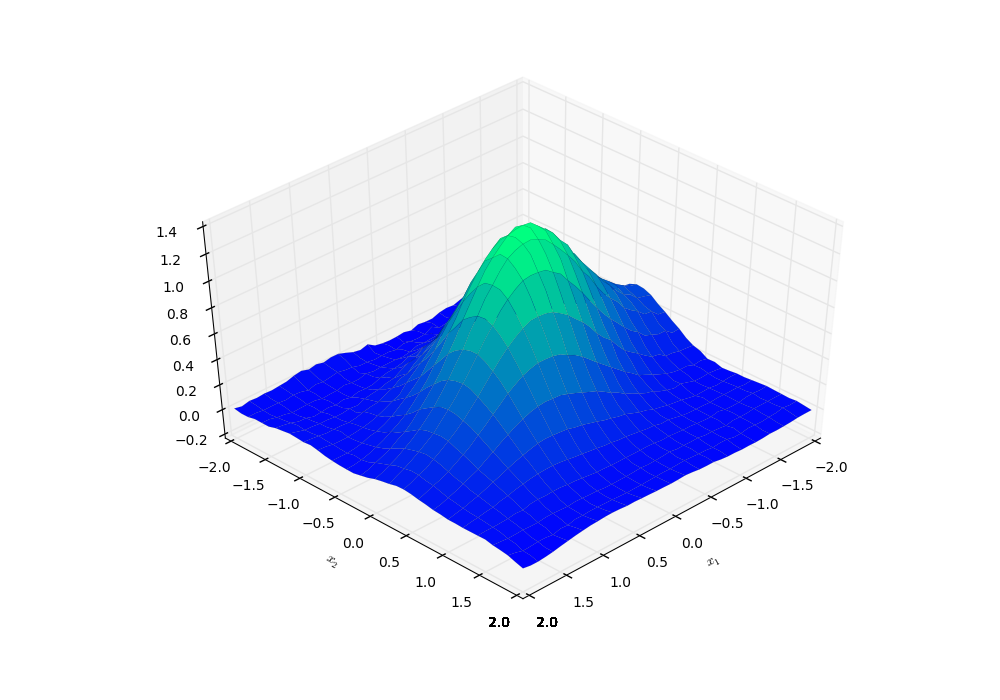
\includegraphics[width=\textwidth]{plot/ex2_6_2000.png}\vspace{-0.5cm}
				\caption{Output after 2000 cycles.}
			\end{subfigure}
   			\caption{\vspace{-0.1cm} 2D graphs of the output of network where the data set is in a randomized order, with $\eta = 0.001$ and 60 hidden nodes.}\vspace{-0.2cm}
  		\end{figure}
		We also tried a learning rate of 0.0001, to see what happens. This does not converge within 2000 cycles, it is too slow. 
		\begin{figure}[h!]
			\centering
			\begin{subfigure}[b]{0.45\textwidth}
				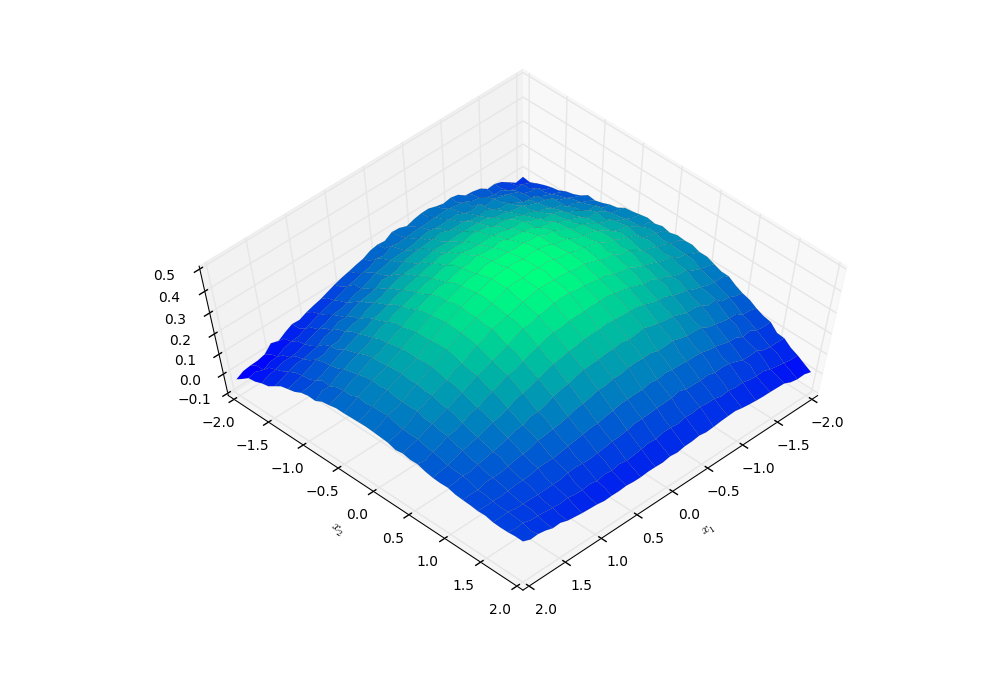
\includegraphics[width=\textwidth]{plot/ex2_6_alt50.png}\vspace{-0.5cm}
				\caption{Output after 50 cycles.}
			\end{subfigure}
			\begin{subfigure}[b]{0.45\textwidth}
				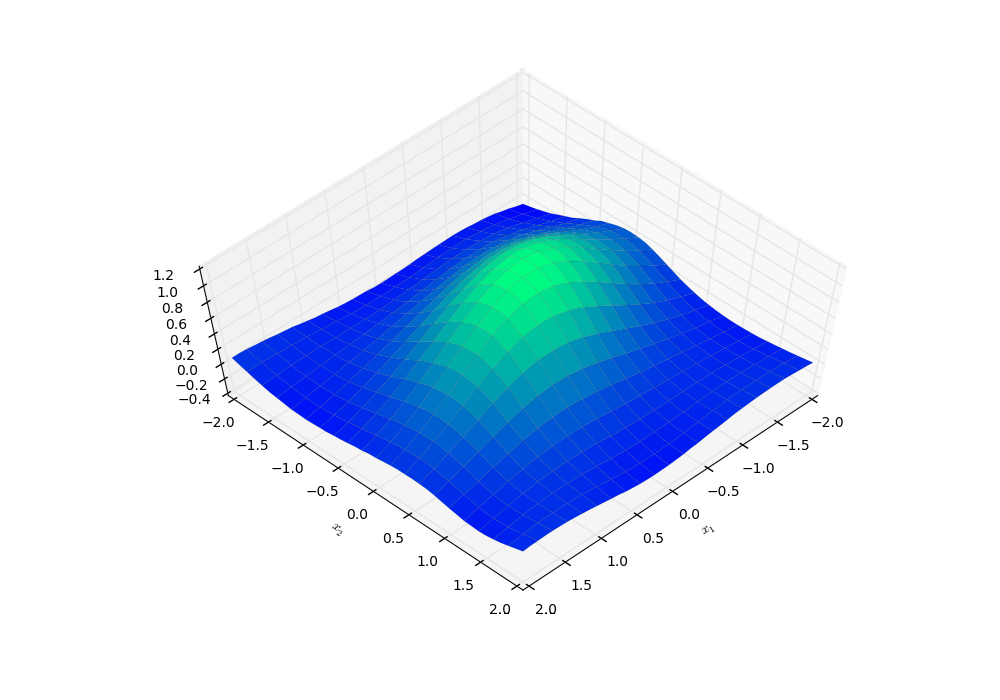
\includegraphics[width=\textwidth]{plot/ex2_6_alt2000.png}\vspace{-0.5cm}
				\caption{Output after 2000 cycles.}
			\end{subfigure}
   			\caption{\vspace{-0.1cm} 2D graphs of the output of network where the data set is in a randomized order, with $\eta = 0.0001$ and 80 hidden nodes}\vspace{-0.2cm}
  		\end{figure}
		
\end{enumerate}

%\vfill

\section{EM and doping}
\begin{enumerate}
	\item \begin{figure}[h!]
   			\centering
   			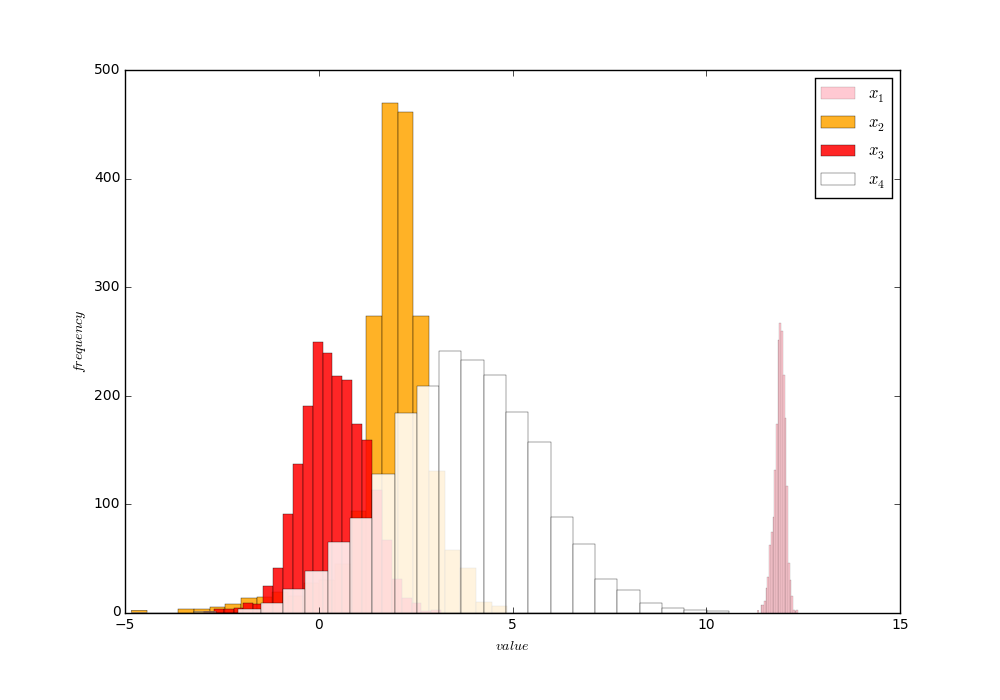
\includegraphics[width=0.46\textwidth]{hist_x.png}\vspace{-0.6cm}
   			\caption{\vspace{-0.1cm} Histogram of the data, different colorings for different $x_i$}\vspace{-0.2cm}
  		\end{figure}
		\begin{figure}[h!]
			\centering
			\begin{subfigure}[b]{0.45\textwidth}
				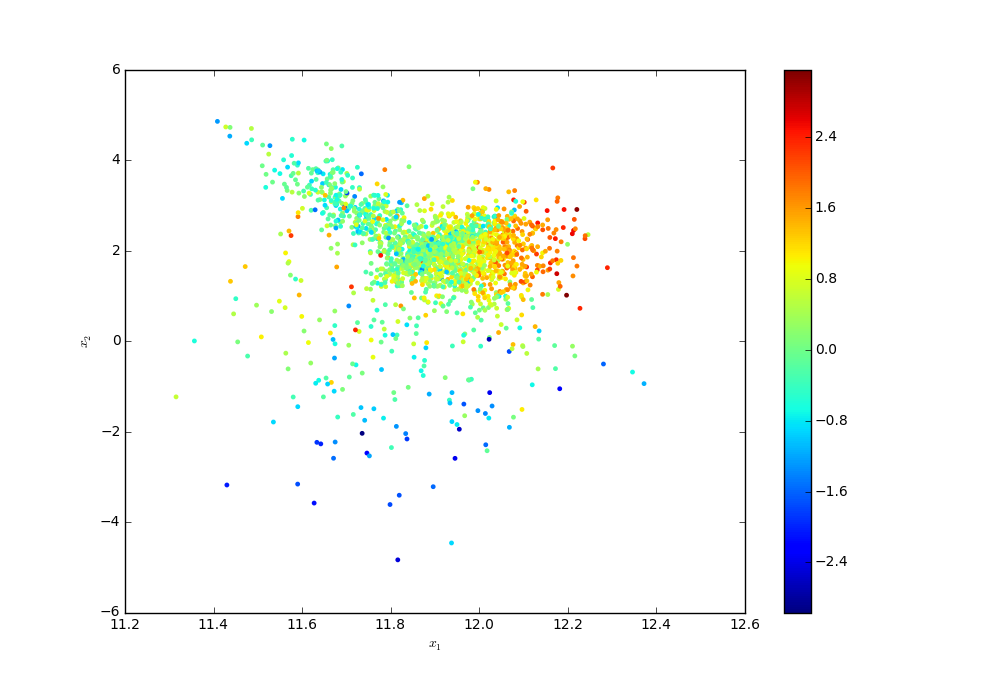
\includegraphics[width=\textwidth]{scatter_x3.png}\vspace{-0.5cm}
				\caption{Colored based on $x_3$.}
			\end{subfigure}
			\begin{subfigure}[b]{0.45\textwidth}
				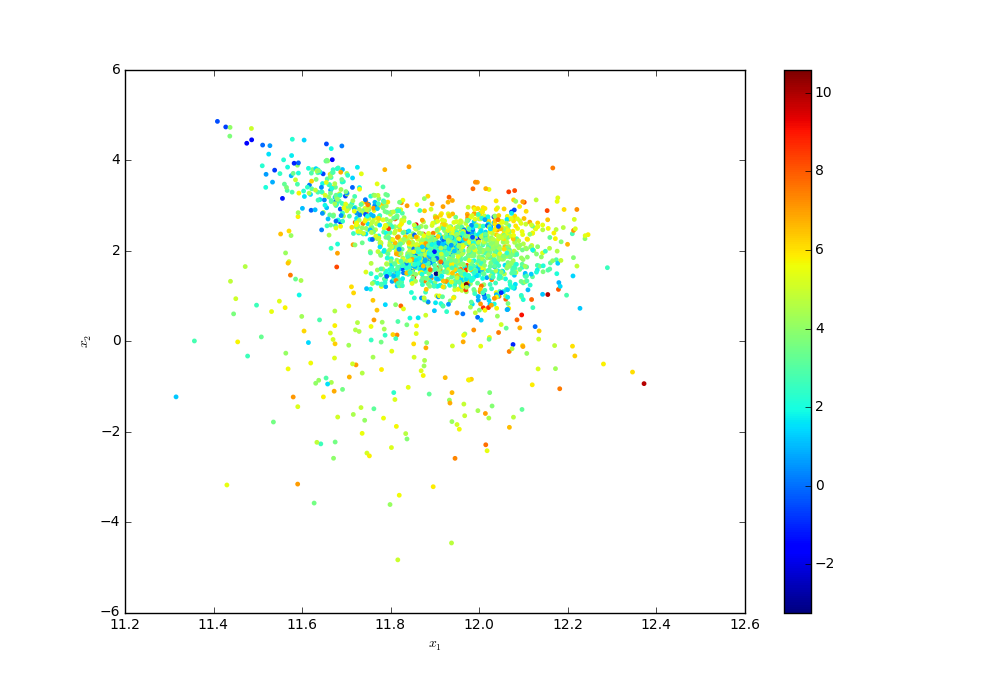
\includegraphics[width=\textwidth]{scatter_x4.png}\vspace{-0.5cm}
				\caption{Colored based on $x_4$.}
			\end{subfigure}
			\begin{subfigure}[b]{0.45\textwidth}
				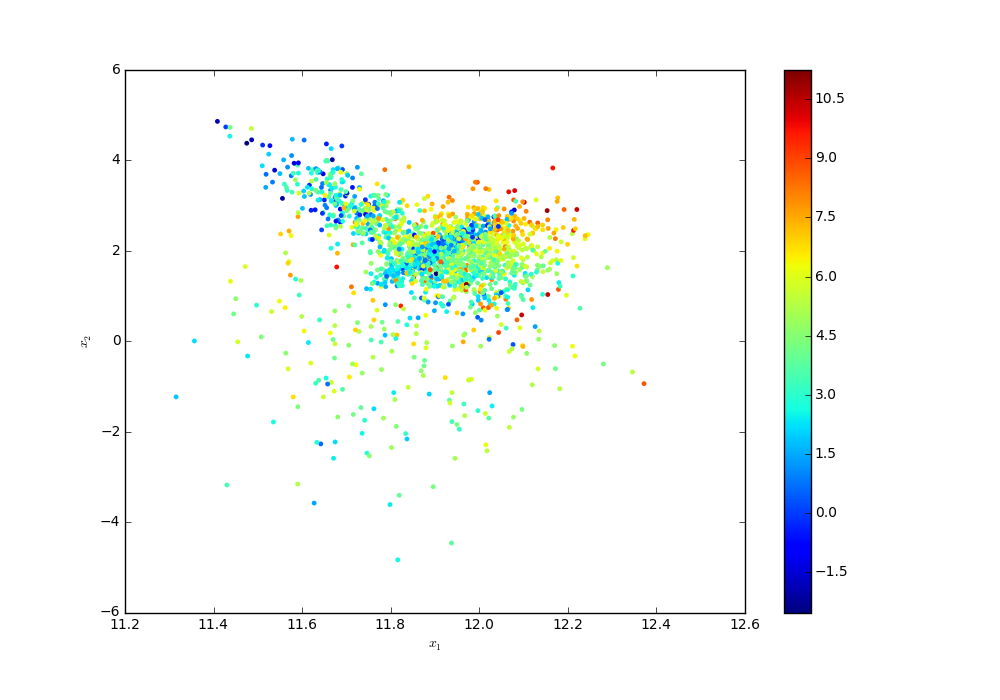
\includegraphics[width=\textwidth]{scatter_x3plusx4.png}\vspace{-0.5cm}
				\caption{Colored based on $x_3 + x_4$.}
			\end{subfigure}
   			\caption{\vspace{-0.1cm} Scatter plot of data points on axes $x_1$ and $x_2$.}\vspace{-0.2cm}
  		\end{figure}
		The histograms in Figure 3.1 show the distribution of each variable. We think there are 3-4 classes, as far as we can tell from the scatter plots in Figure 3.2. In Figure 3.3 our estimation of the clusters is shown. We chose these clusters because these are groups of similar sample size, with different densities but the same distance between data points within each group. In the smallest group, the most dense, there is a strong positive correlation between $x_1$ and $x_2$, and we believe this is the group of athletes that have substance X in their blood.
		\begin{figure}[h!]
   			\centering
   			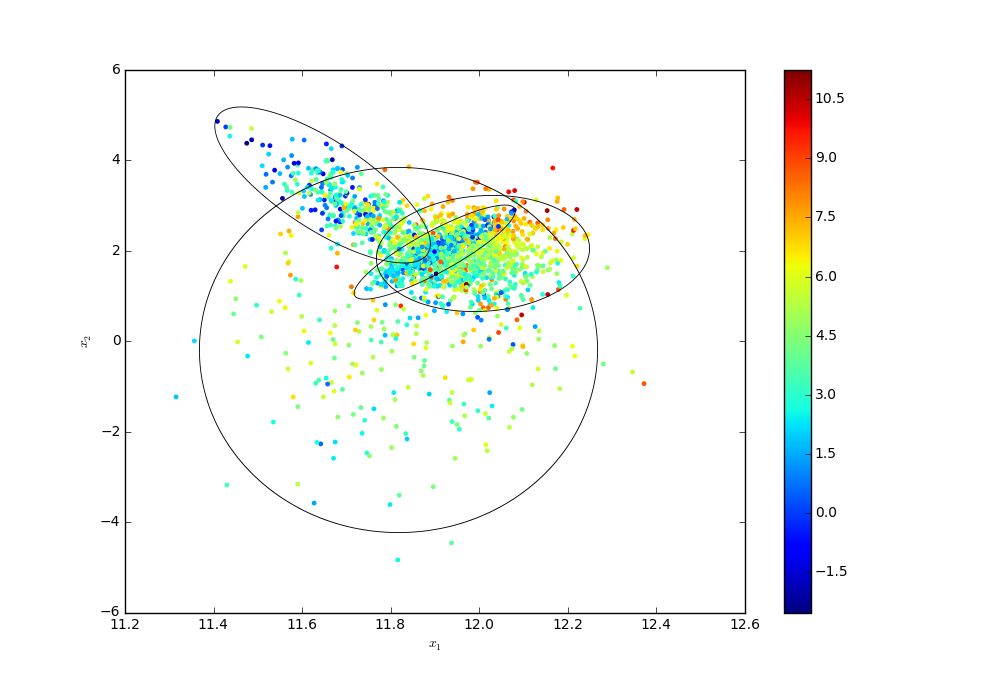
\includegraphics[width=0.44\textwidth]{scatter_x3plusx4_clusters.png}\vspace{-0.6cm}
   			\caption{\vspace{-0.1cm} Figure 3.2(c) with our estimation of the class distributions drawn over it.}\vspace{-0.2cm}
  		\end{figure}
	\item The EM algorithm is divided in the following steps:
		\begin{enumerate}
			\item Set initial values: $K$, $\pi_k$, $\boldsymbol{\mu}_k$, $\boldsymbol{\Sigma}_k$ and evaluate the initial value for the log likelihood.
			\item \textbf{E step}: \begin{equation*}
							\gamma(z_{nk}) = \frac{\pi_k \mathcal{N}(\boldsymbol{x}_n \big\vert \boldsymbol{\mu}_k, \boldsymbol{\Sigma}_k)}{\sum_{j=1}^K \pi_j \mathcal{N}(\boldsymbol{x}_n \big\vert \boldsymbol{\mu}_j, \boldsymbol{\Sigma}_j)}
							\end{equation*}
			\item \textbf{M step:} Re-estimate parameters:
				\begin{align*} 
				\boldsymbol{\mu}_k^{\text{new}} &= \frac{1}{N_k} \sum_1^N \gamma(z_{nk}) \boldsymbol{x}_n\\
				\boldsymbol{\Sigma}_k^{\text{new}} &= \frac{1}{N_k} \sum_1^N \gamma(z_{nk} (\boldsymbol{x}_n - \boldsymbol{\mu}_k^{\text{new}}) (\boldsymbol{x}_n - \boldsymbol{\mu}_k^{\text{new}})^T\\
				\pi_k^{\text{new}} &= \frac{N_k}{N}\\
				\text{where} \hspace{0.6cm} &\\
				N_k &= \sum_1^N \gamma(z_{nk})
				\end{align*}
			\item Evaluate the log likelihood:
				\begin{equation*}
				\ln p(\boldsymbol{X} \big\vert \boldsymbol{\mu}, \boldsymbol{\Sigma}, \boldsymbol{\pi}) = \sum_1^N \ln \bigg\{ \sum_1^K \pi_k \mathcal{N}(\boldsymbol{x}_n \big\vert \boldsymbol{\mu}_k, \boldsymbol{\Sigma}_k) \bigg\}
				\end{equation*}
		\end{enumerate}
	\item \begin{figure}[h!]
   			\centering
   			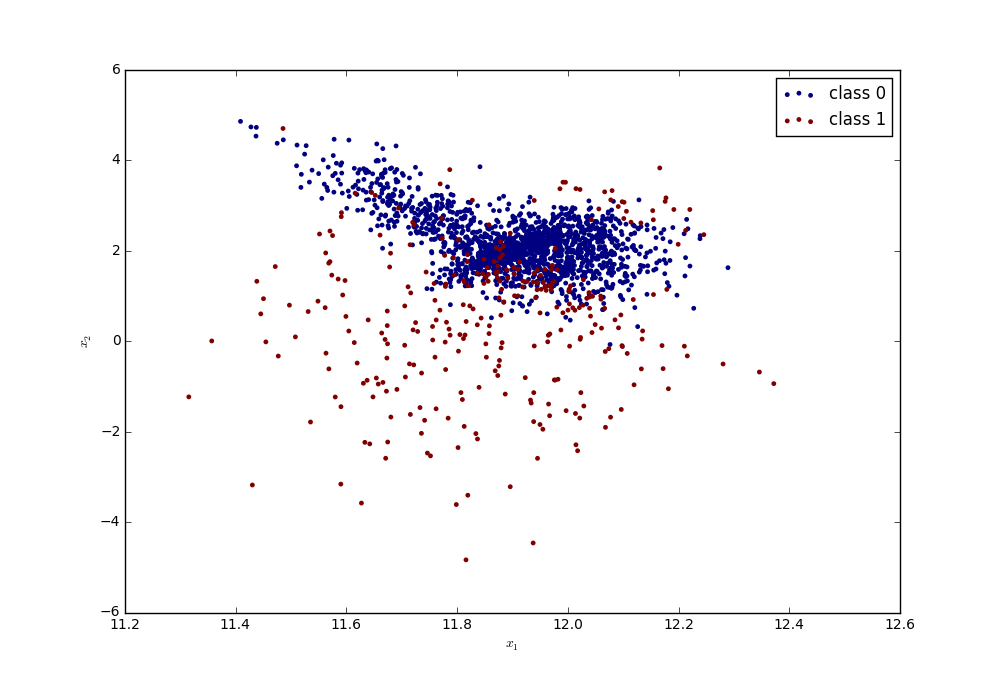
\includegraphics[width=0.6\textwidth]{ex3plots/class_2_100.png}\vspace{-0.6cm}
   			\caption{\vspace{-0.1cm} Scatter plot of data points colored according to most probable component, $K = 2$.}\vspace{-0.2cm}
  		\end{figure}
		The correlation coefficients:
		\begin{equation*}
			\rho_{12} = \frac{\text{cov}[x_1,x_2]}{\sqrt{\text{var}[x_1]\text{var}[x_2]}}
		\end{equation*}
		of the components are -0.5244 for class 0 and 0.1338 for class 1. None of these show the characteristic positive correlation for $\{x_1,x_2\}$. Different initializations do not alter the classes much, all cases we got similar clusters.
	\item \begin{figure}[h!]
   			\centering
   			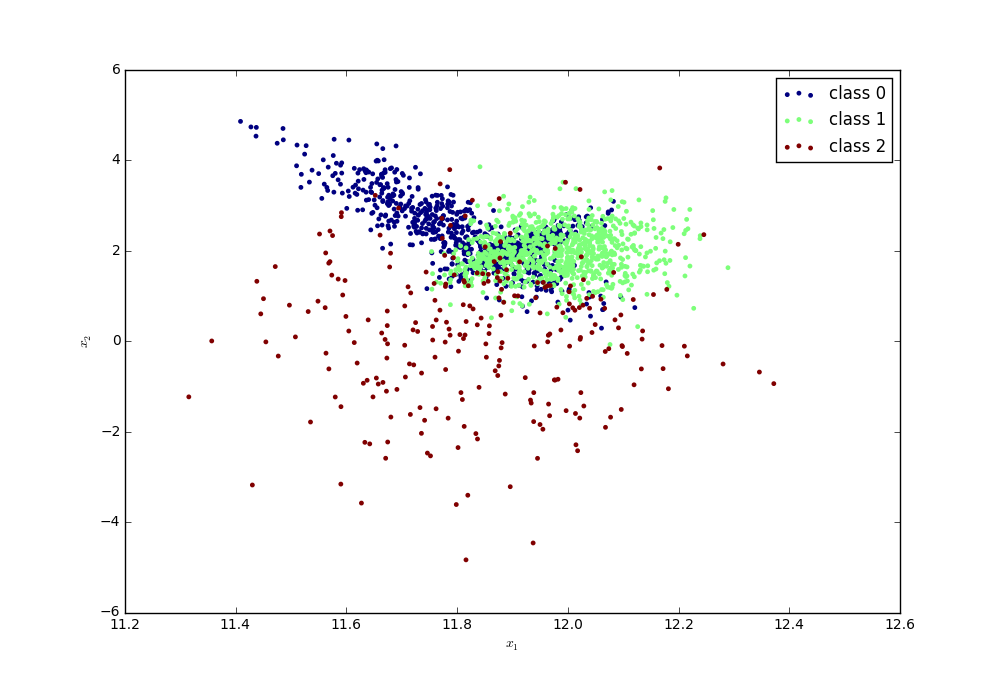
\includegraphics[width=0.6\textwidth]{ex3plots/class_3_100.png}\vspace{-0.6cm}
   			\caption{\vspace{-0.1cm} Scatter plot of data points colored according to most probable component, $K = 3$.}\vspace{-0.2cm}
  		\end{figure}
		The correlation coefficients of the components are 0.0005 for class 0, 0.1146 for class 1 and -0.7181 for class 2. None of these show the characteristic positive correlation for $\{x_1,x_2\}$.
		\begin{figure}[h!]
   			\centering
   			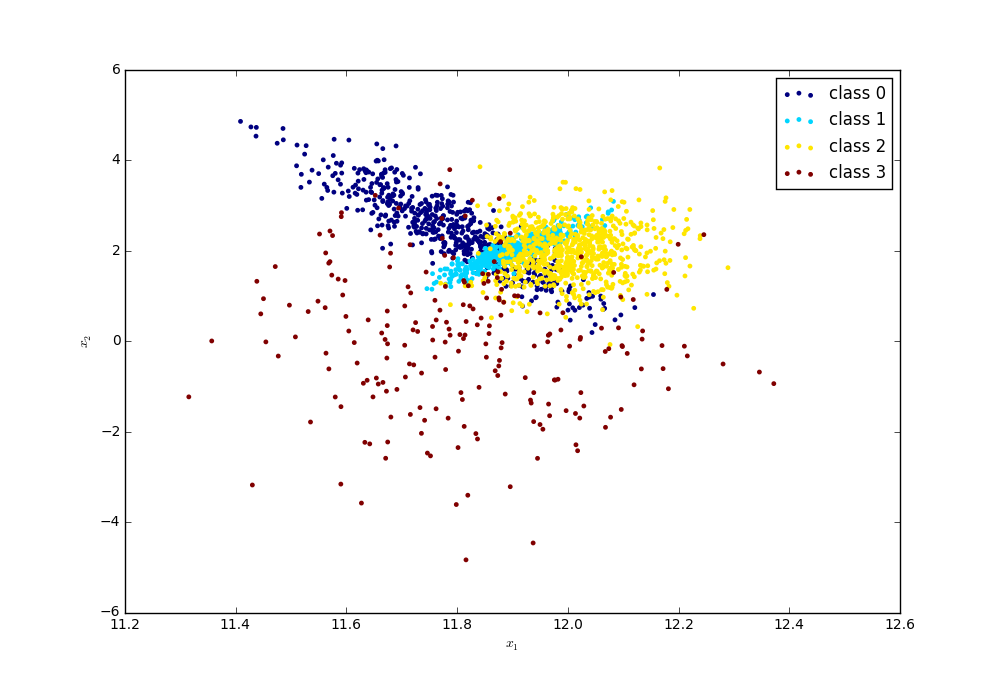
\includegraphics[width=0.6\textwidth]{ex3plots/class_4_100.png}\vspace{-0.6cm}
   			\caption{\vspace{-0.1cm} Scatter plot of data points colored according to most probable component, $K = 4$.}\vspace{-0.2cm}
  		\end{figure}
		The correlation coefficients of the components are -0.9102 for class 0, 0.9102 for class 1, 0.0495 for class 2 and -0.1077 for class 3. Class 1 displays the characteristic positive correlation for $\{x_1,x_2\}$. There are 453 data points in class 1, which corresponds to 22.65\% and thus around 1 in 5 users. We deem the rumoured 1-in-5 estimate for users of X credible.
	\item Subject C is classified in class 1, which corresponds to the group of users of X. Subjects A and D are both classified in class 2, which is the largest group of users. Subject B is classified in class 0, the class with the strong negative correlation. We calculated the likelihoods for every subject, and found that while A, C and D had small probabilities for three classes but a high probability for the class they were put in, and corresponding with this also a likelihood of around 0.1-0.2, subject B was substantially different. Subject B had small probabilities for all classes, and a likelihood of 0.0000009, incredibly small, and was thus hard to classify. This is why we conclude that subject B is most likely the fraud.
\end{enumerate}

%\vfill

\section{Handwritten digit recognition}
\begin{enumerate}
	\item \begin{figure}[h!]
			\centering
			\begin{subfigure}[b]{0.26\textwidth}
				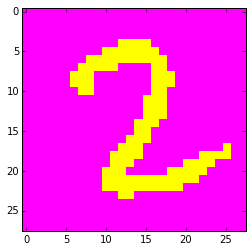
\includegraphics[width=\textwidth]{digits/normaletwee.png}\vspace{-0.4cm}
				\caption{A two.}
			\end{subfigure}
			\begin{subfigure}[b]{0.26\textwidth}
				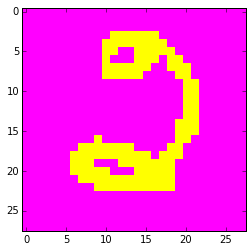
\includegraphics[width=\textwidth]{digits/cooletwee.png}\vspace{-0.4cm}
				\caption{A different two.}
			\end{subfigure}
			\begin{subfigure}[b]{0.26\textwidth}
				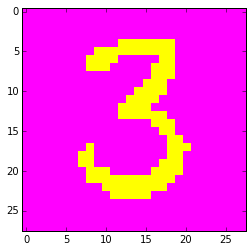
\includegraphics[width=\textwidth]{digits/skondrie.png}\vspace{-0.4cm}
				\caption{A three.}
			\end{subfigure}
			\begin{subfigure}[b]{0.26\textwidth}
				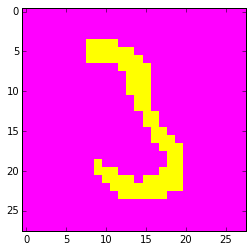
\includegraphics[width=\textwidth]{digits/rare3.png}\vspace{-0.4cm}
				\caption{A sloppy written three.}
			\end{subfigure}
			\begin{subfigure}[b]{0.26\textwidth}
				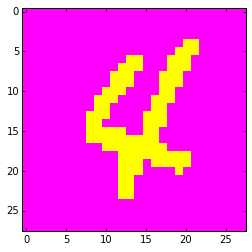
\includegraphics[width=\textwidth]{digits/via.png}\vspace{-0.4cm}
				\caption{A four.}
			\end{subfigure}
			\begin{subfigure}[b]{0.26\textwidth}
				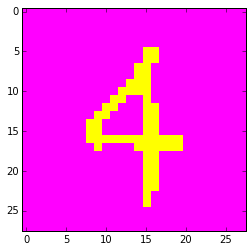
\includegraphics[width=\textwidth]{digits/dichtvier.png}\vspace{-0.4cm}
				\caption{A different four.}
			\end{subfigure}
   			\caption{\vspace{-0.1cm} Examples of handwritten digits in the dataset, binary images displayed in a happy springy colormap.}\vspace{-0.2cm}
  		\end{figure}
		We would need class prototypes that represent the different ways of writing the same number. As shown in Figure 4.1, this might prove to be difficult, since some people write a $2$ with a small loop at the bottom, or even at the top, while others do not. The number $3$ can be really round, or more like a straight banana-shape. The number $4$ can be either open or closed at the top. These different handwritings may complicate dividing the images into classes. However, with the right prototypes, we think at least most of the numbers can be classified correctly, because there are also more consistent differences.
	\item 
		
\end{enumerate}

\end{document}